%
% Copyright 2018 Joel Feldman, Andrew Rechnitzer and Elyse Yeager.
% This work is licensed under a Creative Commons Attribution-NonCommercial-ShareAlike 4.0 International License.
% https://creativecommons.org/licenses/by-nc-sa/4.0/
%
\questionheader{ex:s3.4.2}


%%%%%%%%%%%%%%%%%%
\subsection*{\Conceptual}
%%%%%%%%%%%%%%%%%%



\begin{Mquestion}
Suppose $f(x)$ is a function, and we calculated its linear approximation near $x=5$ to be
$f(x) \approx 3x-9$.
\begin{enumerate}[(a)]
\item What is $f(5)$?
\item What is $f'(5)$?
\item What is $f(0)$?
\end{enumerate}
\end{Mquestion}
\begin{hint}
The linear approximation $L(x)$ is chosen so that $f(5)=L(5)$ and $f'(5)=L'(5)$.
\end{hint}
\begin{answer}
(a) $f(5)=6$\qquad
(b) $f'(5)=3$\qquad
(c) not enough information to know
\end{answer}
\begin{solution}
The linear approximation is $L(x)=3x-9$. Since we're approximating at $x=5$, $f(5)=L(5)$, and $f'(5)=L'(5)$. However, there is no guarantee that $f(x)$ and $L(x)$ have the same value when $x \neq 5$. So:\\
(a) $f(5)=L(5)=6$\\
(b) $f'(5)=L'(5)=3$\\
(c) there is not enough information to find $f(0)$.
\end{solution}


\begin{Mquestion}
The curve $y=f(x)$ is shown below. Sketch the linear approximation of $f(x)$ about $x=2$.
\begin{center}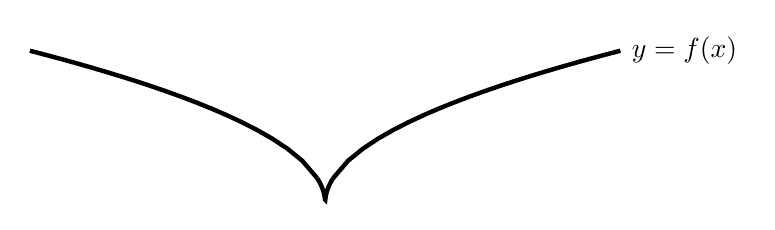
\begin{tikzpicture}
\YEaxis{4}{2.5}
\draw[ultra thick] plot[domain=-3.75:-.1, samples=20](\x,{sqrt(abs(\x))});
\draw[ultra thick] plot[domain=.1:3.75, samples=20](\x,{sqrt(abs(\x))}) node[right]{$y=f(x)$};
\draw [ultra thick]plot[domain=-.1:.1, samples=50](\x,{sqrt(abs(\x))});
\YExcoord{2}{2};
\end{tikzpicture}\end{center}
\end{Mquestion}
\begin{hint}
The graph of the linear approximation is a line, passing through $(2,f(2))$, with slope $f'(2)$.
\end{hint}
\begin{answer}
\begin{center}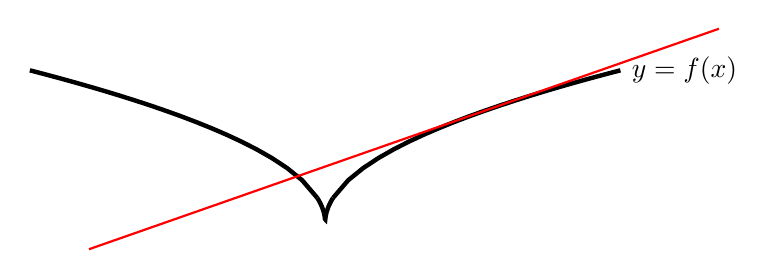
\begin{tikzpicture}
\YEaxis{4}{2.5}
\draw[ultra thick] plot[domain=-3.75:-.1, samples=20](\x,{sqrt(abs(\x))});
\draw[ultra thick] plot[domain=.1:3.75, samples=20](\x,{sqrt(abs(\x))}) node[right]{$y=f(x)$};
\draw [ultra thick]plot[domain=-.1:.1, samples=50](\x,{sqrt(abs(\x))});
\YExcoord{2}{2};
\draw[thick, red] plot[domain=-3:5] (\x,{sqrt(2)+0.35*(\x-2)});
\end{tikzpicture}\end{center}
The linear approximation is shown in red.
\end{answer}
\begin{solution}
The linear approximation is a line, passing through $(2,f(2))$, with slope $f'(2)$.
That is, the linear approximation to $f(x)$ about $x=2$ is the tangent line to $f(x)$ at $x=2$. It is shown below in red.
\begin{center}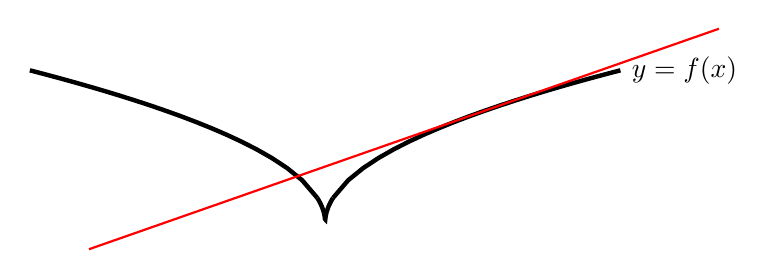
\begin{tikzpicture}
\YEaxis{4}{2.5}
\draw[ultra thick] plot[domain=-3.75:-.1, samples=20](\x,{sqrt(abs(\x))});
\draw[ultra thick] plot[domain=.1:3.75, samples=20](\x,{sqrt(abs(\x))}) node[right]{$y=f(x)$};
\draw [ultra thick]plot[domain=-.1:.1, samples=50](\x,{sqrt(abs(\x))});
\YExcoord{2}{2};
\draw[thick, red] plot[domain=-3:5] (\x,{sqrt(2)+0.35*(\x-2)});
\end{tikzpicture}\end{center}

\end{solution}





\begin{question}
What is the linear approximation of the function $f(x)=2x+5$ about $x=a$?
\end{question}
\begin{hint}
It's an extremely accurate approximation.
\end{hint}
\begin{answer}
$f(x)=2x+5$
\end{answer}
\begin{solution}
For any constant $a$, $f(a)=(2a+5)$, and $f'(a)=2$, so our approximation gives us
\[f(x) \approx (2a+5)+2(x-a)=2x+5\]

Since $f(x)$ itself is a linear function, the linear approximation is actually just $f(x)$ itself. As a consequence, the linear approximation is perfectly accurate for all values of $x$.
\end{solution}



%%%%%%%%%%%%%%%%%%
\subsection*{\Procedural}
%%%%%%%%%%%%%%%%%%



\begin{Mquestion}
Use a linear approximation to estimate $\log(x)$ when $x=0.93$. Sketch the curve $y=f(x)$ and your linear approximation.

(Remember that in CLP-1 we use $\log x$ to mean the natural logarithm of $x$, $\log_e x$.)
\end{Mquestion}
\begin{hint}
You'll need to centre your approximation about some $x=a$, which should have two properties: you can easily compute $\log(a)$, and $a$ is close to $0.93$.
\end{hint}
\begin{answer}
$\log(0.93) \approx -0.07$
 \begin{center}\begin{tikzpicture}
 \YEaaxis{1.5}{3.5}{1}{2}
 \draw[thick] plot[domain=0.25:3](\x,{ln \x}) node[right]{$y=f(x)$};
 \draw[thick, red] plot[domain=-.5:3] (\x,{\x-1}) node[ right]{$y=x-1$};
 \YExcoord{1}{1};
 \end{tikzpicture}\end{center}
\end{answer}
\begin{solution}
We have no idea what $f(0.93)$  is, but 0.93  is pretty close to 1, and we definitely know $f(1)$. The linear approximation of $f(x)$ about $x=1$ is given by
\begin{align*}
f(x) &\approx f(1)+f'(1)(x-1)
\intertext{So, we calculate:}
f(1)&=\log(1)=0\\
f'(x)&=\frac{1}{x}\\
f'(1)&=\frac{1}{1}=1
\intertext{Therefore,}
f(x) &\approx 0+1(x-1)=x-1
\intertext{When $x=0.93$:}
f(0.93) &\approx 0.93-1=-0.07
\end{align*}
 \begin{center}\begin{tikzpicture}
 \YEaaxis{1.5}{3.5}{1}{2}
 \draw[thick] plot[domain=0.25:3](\x,{ln \x}) node[right]{$y=f(x)$};
 \draw[thick, red] plot[domain=-.5:3] (\x,{\x-1}) node[ right]{$y=x-1$};
 \YExcoord{1}{1};
 \end{tikzpicture}\end{center}
\end{solution}




\begin{Mquestion}
Use a linear approximation to estimate $\sqrt{5}$.
\end{Mquestion}
\begin{hint}
Approximate the function $f(x) = \sqrt{x}$.
\end{hint}
\begin{answer}
$\sqrt{5} \approx \dfrac{9}{4}$
\end{answer}
\begin{solution}
We approximate the function $f(x)=\sqrt{x}$ about $x=4$, since 4 is a perfect square and it is close to 5.
\begin{align*}
f(4)&=\sqrt{4}=2\\
f'(x)&=\frac{1}{2\sqrt{x}} \qquad \Rightarrow \qquad f'(4)=\frac{1}{2\sqrt{4}}=\frac{1}{4}\\
f(x) &\approx f(4)+f'(4)(x-4)=2+\frac{1}{4}(x-4)\\
f(5)&\approx 2+\frac{1}{4}(5-4)=\frac{9}{4}
\end{align*}
We estimate $\sqrt{5}\approx\dfrac{9}{4}$.

Remark: $\left(\dfrac{9}{4}\right)^2=\dfrac{81}{16}$, which  is pretty close to $\dfrac{80}{16}=5$. Our approximation seems pretty good.
\end{solution}






\begin{question}
Use a linear approximation to estimate $\sqrt[5]{30}$
\end{question}
\begin{hint}
Approximate the function $f(x)=\sqrt[5]{x}$.
\end{hint}
\begin{answer}
$\sqrt[5]{30}\approx \dfrac{79}{40}$
\end{answer}
\begin{solution}
We approximate the function $f(x)=\sqrt[5]{x}$. We need to centre the approximation about some value $x=a$ such that we know $f(a)$ and $f'(a)$, and $a$ is not too far from $30$.
\begin{align*}
f(x)&=\sqrt[5]{x}=x^{\frac{1}{5}}\\
f'(x)&=\frac{1}{5}x^{-\frac{4}{5}}=\frac{1}{5\sqrt[5]{x}^4}
\intertext{$a$ needs to be a number whose fifth root we know. Since $\sqrt[5]{32}=2$, and 32 is reasonably close to 30, $a=32$ is a great choice.}
f(32)&=\sqrt[5]{32}=2\\
f'(32)&=\frac{1}{5\cdot 2^4}=\frac{1}{80}
\intertext{The linear approximation of $f(x)$ about $x=32$ is}
f(x) &\approx 2+\frac{1}{80}(x-32)
\intertext{When $x=30$:}
f(30) &\approx 2+\frac{1}{80}(30-32)=2-\frac{1}{40}=\frac{79}{40}
\end{align*}
We estimate $\sqrt[5]{30}\approx \dfrac{79}{40}$.

Remark: $\dfrac{79}{40} = 1.975$, while $\sqrt[5]{30} \approx 1.97435$. This is a  decent estimation.
\end{solution}





%%%%%%%%%%%%%%%%%%
\subsection*{\Application}
%%%%%%%%%%%%%%%%%%


%\begin{question}
%In this question, we want to estimate $\tan(1)$.
%\begin{enumerate}[(a)]
%\item Use a constant approximation about $x=\dfrac{\pi}{3}$ to estimate $\tan(1)$.
%\item Use a linear approximation to estimate $\sqrt{3}$ as a decimal, and use this to %estimate $\tan(1)$ as a combination of integer fractions and pi.
%\item Compare your estimation for $\tan(1)$ to its value from a calculator.
%\end{enumerate}
%\end{question}
%\begin{hint}
%What is the closest perfect square to 3?
%\end{hint}
%\begin{answer}
%\end{answer}
%\begin{solution}
%(a) The linear approximation of
%$f(x)$ about $x=\dfrac{\pi}{3}$ is given by
%\begin{align*}
%f(x) &\approx f\left(\frac{\pi}{3}\right)+f'\left(\frac{\pi}{3}\right)\left(x-\frac{\pi}{3}\right)
%\intertext{So, we calculate:}
%f\left(\frac{\pi}{3}\right)&=\sqrt{3}\\
%f'\left(\frac{\pi}{3}\right)&=\sec^2\left(\frac{\pi}{3}\right)=2
%\intertext{Therefore,}
%f(x) &\approx \sqrt{3}+2\left(x-\frac{\pi}{3}\right)=2x-\frac{2}{3}\pi+\sqrt{3}
%\intertext{When $x=1$:}
%f(1) &\approx 2-\frac{2}{3}\pi+\sqrt{3}
%\end{align*}
%(b) Let $g(x)=\sqrt{x}$. We want to estimate $g(3)$, but we only know $g(x)$ when $x$ %is a perfect square. The closest perfect square to 3 is 4. So, we take the linear %approximation of $g(x)$ about $x=4$.
%\begin{align*}
%g(x) &\approx g(4)+g'(4)(x-4)\\
%g(4)&=\sqrt{4}=2\\
%g'(4)&=\frac{1}{2\sqrt{4}}=\frac{1}{8}
%\intertext{So,}
%g(x) &\approx 2+\frac{1}{8}(x-4)=\frac{1}{8}x+\frac{3}{2}
%\intertext{When $x=3$,}
%g(3)&\approx \frac{3}{8}+\frac{3}{2}=\frac{15}{8}
%\intertext{Since we estimated $\tan(1) \approx 2-\dfrac{2}{3}\pi+\sqrt{3}$,}
%\tan(1)&\approx 2-\frac{2}{3}\pi +\frac{15}{8}=\frac{31}{8}-\frac{2}{3}\pi
%\end{align*}
%(c) We estimated $\tan(1) \approx \dfrac{31}{8}-\dfrac{2}{3}\pi \approx 1.78$, and a %calculator estimates $\tan(1) \approx 1.56$.
%\end{solution}



\begin{Mquestion}
Use a linear approximation to estimate $10.1^3$, then compare your estimation with the actual value.
\end{Mquestion}
\begin{hint}
Approximate the function $f(x)=x^3$.
\end{hint}
\begin{answer}
$10.1^3 \approx 1030$, $10.1^3 = 1030.301$
\end{answer}
\begin{solution}
If $f(x)=x^3$, then $f(10.1)=10.1^3$, which is the value we want to estimate. Let's take the linear approximation of $f(x)$ about $x=10$:
\begin{align*}
f(10)&=10^3=1000\\
f'(x)&=3x^2\\
f'(10)&=3(10^2)=300\\
f(a) &\approx f(10)+f'(10)(x-10)\\
&=1000+300(x-10)\\
f(10.1)& \approx 1000+300(10.1-10)=1030
\end{align*}
We estimate $10.1^3 \approx 1030$. If we calculate $10.1^3$ exactly (which is certainly possible to do by hand), we get 1030.301.

Remark: in the previous subsection, we used a constant approximation to estimate $10.1^3 \approx 1000$. That approximation was easy to do in your head, in a matter of seconds. The linear approximation is more accurate, but not much faster than simply calculating $10.1^3$.
\end{solution}


\begin{question}
Imagine $f(x)$ is some function, and you want to estimate $f(b)$. To do this, you choose a value $a$ and take an approximation (linear or constant) of $f(x)$ about $a$. Give an example of a function $f(x)$, and values $a$ and $b$, where the constant approximation gives a more accurate estimation of $f(b)$ than the linear approximation.
\end{question}
\begin{hint}
One possible choice of $f(x)$ is $f(x)=\sin x$.
\end{hint}
\begin{answer} There are many possible answers. One is $f(x)=\sin x$, $a=0$, and $b=\pi$.
\end{answer}
\begin{solution}
There are many possible answers. One is:
\[f(x)=\sin x \qquad a=0 \qquad b=\pi \]
We know that $f(\pi)=0$ and $f(0)=0$. Using a constant approximation of $f(x)$ about $x=0$, our estimation is $f(\pi)\approx f(0)=0$, which is exactly the correct value. However, is we make a linear approximation of $f(x)$ about $x=0$, we get
\[
f(\pi) \approx f(0)+f'(0)(\pi-0)=\sin(0)+\cos(0)\pi=\pi
\]
which is not exactly the correct value.
\begin{center}\begin{tikzpicture}
\YEaaxis{2}{5}{1.5}{4.5}
\YExcoord{3.14}{\pi};
\draw[ultra thick] plot[domain=-1.75:3.75, samples=100](\x,{sin(\x r)}) node[right]{$y=f(x)$};
\draw[thick, red] (-1,0)--(4,0) node[above right]{const};
\draw[thick, blue] (-1.5,-1.5)--(3.25,3.25) node[ right]{linear};
\end{tikzpicture}\end{center}
Remark: in reality, we wouldn't estimate $\sin(\pi)$, because we know its value exactly. The purpose of this problem is to demonstrate that fancier approximations are not \emph{always} more accurate. At the end of this section, we'll talk about how to bound the error of your estimations, to make sure that you are finding something sufficiently accurate.
\end{solution}


\begin{question}
The function
\[L(x)=\frac{1}{4}x+\frac{4\pi-\sqrt{27}}{12}\]
is the linear approximation of $f(x)=\arctan x$ about what point $x=a$?
\end{question}
\begin{hint}
Compare the derivatives.
\end{hint}
\begin{answer}
$a=\sqrt{3}$
\end{answer}
\begin{solution}
The linear approximation $L(x)$ of $f(x)$ about $x=a$ is chosen so that $L(a)=f(a)$
and $L'(a)=f'(a)$. So,
\begin{align*}
L'(a)&= f'(a)=\dfrac{1}{1+a^2}\\
\frac{1}{4}&=\frac{1}{1+a^2}\\
a&=\pm\sqrt{3}
\intertext{We've narrowed down $a$ to $\sqrt{3}$ or $-\sqrt{3}$.
Recall the linear approximation of $f(x)$ about $x=a$ is $f(a)+f'(a)(x-a),$
so its constant term is $f(a)-af'(a)=\arctan(a)-\dfrac{a}{1+a^2}$. We compute this for $a=\sqrt{3}$ and $a=-\sqrt{3}$.}
a=\sqrt{3}:~&~\arctan\left(a\right)-\frac{a}{1+a^2}
=\arctan\left(\sqrt{3}\right)-\frac{\sqrt{3}}{1+\left(\sqrt{3}\right)^2}=\frac{\pi}{3}-\frac{\sqrt{3}}{4}=\frac{4\pi-\sqrt{27}}{12}\\
a=-\sqrt{3}:~&~\arctan\left(a\right)-\frac{a}{1+a^2}
=\arctan\left(-\sqrt{3}\right)-\frac{-\sqrt{3}}{1+\left(-\sqrt{3}\right)^2}=-\frac{\pi}{3}+\frac{\sqrt{3}}{4}=\frac{-4\pi+\sqrt{27}}{12}
\intertext{So, when $a=\sqrt{3}$,}
L(x)&=\frac{1}{4}x+\frac{4\pi-\sqrt{27}}{12}
\end{align*}
and this does not hold when $a=-\sqrt{3}$. We conclude $a=\sqrt{3}$.
\end{solution}
